\chapter{MRI in fifteen minutes}
\label{ch:mri}

\begin{tldr}
\begin{itemize}
\item An MRI \textbf{series} is a stack of 2D slices; a knee \textbf{exam} has several series.
\item Each series is cut in one of three directions: \textbf{sagittal} (side view), \textbf{coronal} (front view),
      \textbf{axial} (cross-section).
\item The scanner settings (the \textbf{sequence}) decide what is bright. \textbf{Fluid-sensitive, fat-suppressed}
      series make fluid, swelling and tears bright: they are the ones that show most findings.
\item Pixels are small (\ca 0.4\,mm) but slices are thick (\ca 3.5\,mm), and brightness has \textbf{no units}.
\end{itemize}
\end{tldr}

\section{How MRI makes a picture, in three sentences}

The scanner is a strong magnet. Radio pulses make the hydrogen in the body's water and fat send back a weak
signal, and the scanner measures it point by point. How bright a tissue looks depends on how much water and fat
it holds \emph{and} on the timing of the radio pulses, so the same knee can be imaged in very different ways.

\section{Slices and stacks}

\begin{figure}[H]
\centering
\begin{tikzpicture}[x=1mm,y=1mm]
  \foreach \k in {0,...,7} {
    \fill[dark!88, draw=white, line width=0.4pt] ({\k*5},{\k*3}) -- ++(30,0) -- ++(0,30) -- ++(-30,0) -- cycle;
    \fill[white!70!dark] ({\k*5+15},{\k*3+15}) circle (7);
    \fill[dark!88] ({\k*5+15},{\k*3+15}) circle (4.5);
  }
  \draw[decorate, decoration={brace, amplitude=1.5mm}, line width=0.6pt] (35,54) -- (65,54)
     node[midway, above=2mm, font=\footnotesize] {one slice: e.g.\ 384\,$\times$\,384 pixels};
  \draw[decorate, decoration={brace, amplitude=1.5mm, mirror}, line width=0.6pt] (31,-1) -- (66,20)
     node[midway, below right=1mm, font=\footnotesize, align=left] {20--40 slices, one file each\\ \ca 3--4\,mm apart};
  \node[anchor=west, font=\footnotesize, align=left] at (82,38) {\textbf{one pixel} \ca 0.3--0.6\,mm wide\\
     \textbf{one slice} \ca 3--4\,mm thick\\[2mm] \textbf{one series} = the whole stack\\ (one direction, one setting)};
\end{tikzpicture}
\caption{A series is a stack of slices. In the competition files every slice is a separate file.}
\end{figure}

\section{Three directions}

\begin{figure}[H]
\centering
\begin{tikzpicture}[x={(1cm,0cm)}, y={(0.45cm,0.32cm)}, z={(0cm,1cm)}, scale=0.7]
  % a leg-shaped box, x = left-right, y = front-back, z = up-down
  \draw[muted, line width=0.5pt] (0,0,0) -- (4,0,0) -- (4,4,0) -- (0,4,0) -- cycle;
  \draw[muted, line width=0.5pt] (0,0,6) -- (4,0,6) -- (4,4,6) -- (0,4,6) -- cycle;
  \foreach \x/\y in {0/0,4/0,4/4,0/4} \draw[muted, line width=0.5pt] (\x,\y,0) -- (\x,\y,6);
  % planes
  \fill[us, opacity=0.35] (2,0,0) -- (2,4,0) -- (2,4,6) -- (2,0,6) -- cycle;
  \fill[them, opacity=0.35] (0,2,0) -- (4,2,0) -- (4,2,6) -- (0,2,6) -- cycle;
  \fill[third, opacity=0.45] (0,0,3) -- (4,0,3) -- (4,4,3) -- (0,4,3) -- cycle;
  \node[font=\small\bfseries, text=us!80!black, anchor=west] at (2.3,4,5.6) {sagittal};
  \node[font=\small\bfseries, text=them!80!black, anchor=west] at (4.15,2,4.6) {coronal};
  \node[font=\small\bfseries, text=third!70!black, anchor=west] at (4.15,4,3) {axial};
  \draw[-{Stealth}, ink] (-0.8,0,0) -- (0.3,0,0) node[right, font=\scriptsize] {left--right};
  \draw[-{Stealth}, ink] (-0.8,0,0) -- (-0.8,1.4,0) node[above left, font=\scriptsize] {front--back};
  \draw[-{Stealth}, ink] (-0.8,0,0) -- (-0.8,0,1.1) node[above, font=\scriptsize] {up};
\end{tikzpicture}\hspace{6mm}
\begin{minipage}[b]{0.52\linewidth}\small
\textcolor{us}{\textbf{Sagittal}}: slices from left to right. Each slice is a side view. Best for the ACL, the front and back of
the menisci, effusion.\par\medskip
\textcolor{them!85!black}{\textbf{Coronal}}: slices from front to back. Each slice is a front view. Best for the
MCL, the middle of the menisci, medial vs.\ lateral cartilage.\par\medskip
\textcolor{third!75!black}{\textbf{Axial}}: slices from bottom to top. Each slice is a cross-section of the
leg. Best for the kneecap (PF OA), Baker's cyst, synovitis.\par\bigskip
\end{minipage}
\caption{The three directions. Each one shows full detail within its slices and coarse detail across them,
so an exam needs all three.}
\label{fig:planes}
\end{figure}

\begin{figure}[H]
\centering
\begin{subfigure}[t]{0.33\linewidth}\centering
  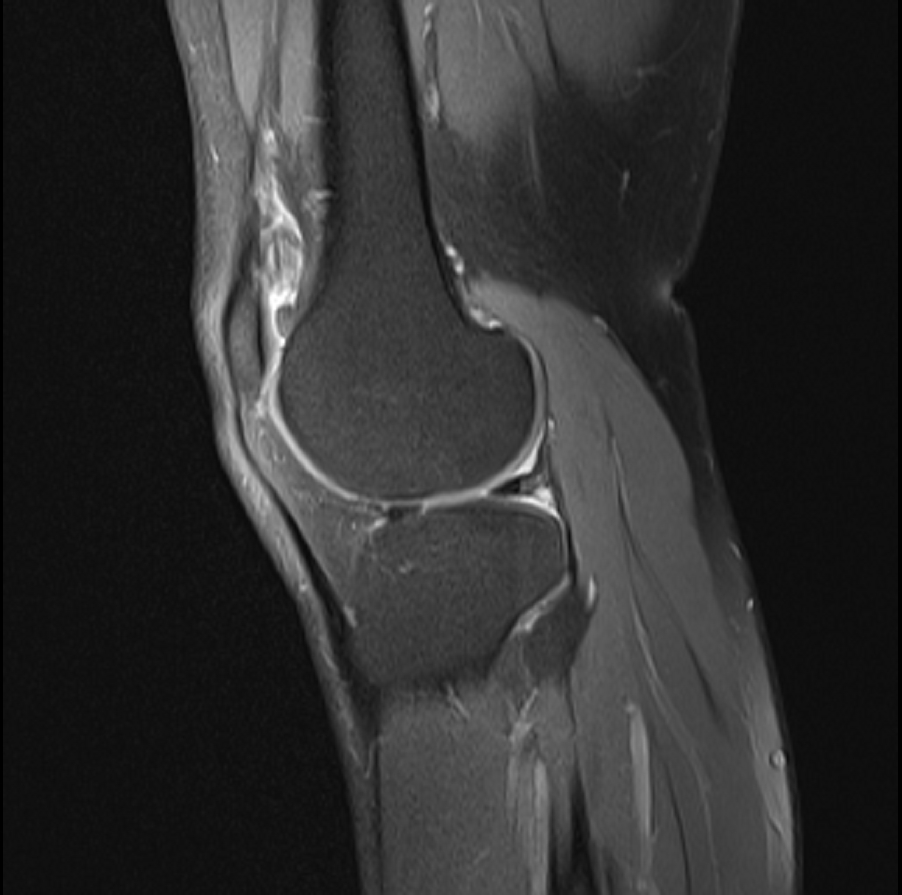
\includegraphics[height=46mm]{img/commons/sag_pd_fs.jpg}
  \caption{Sagittal (front of the knee on the left).}
\end{subfigure}\hfill
\begin{subfigure}[t]{0.25\linewidth}\centering
  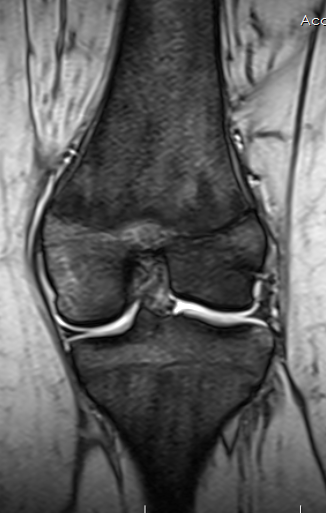
\includegraphics[height=46mm]{img/commons/cor_t2.png}
  \caption{Coronal.}
\end{subfigure}\hfill
\begin{subfigure}[t]{0.33\linewidth}\centering
  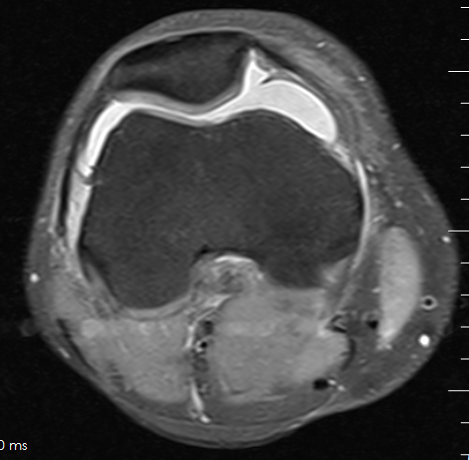
\includegraphics[height=46mm]{img/commons/ax_pd_fs.png}
  \caption{Axial (kneecap at the top).}
\end{subfigure}
\caption{One slice from each direction (three different people). Compare them with the drawings in
Figure~\ref{fig:anatomy}. Images: Ptrump16 and Nevit Dilmen, Wikimedia Commons, CC BY-SA.}
\label{fig:realplanes}
\end{figure}

\section{Sequences: what is bright and what is dark}

The radio-pulse timing is called the \term{sequence}. Knee exams use two families:

\begin{figure}[H]
\centering
\begin{subfigure}[t]{0.42\linewidth}\centering
  \begin{tikzpicture}
    \node[anchor=south west, inner sep=0] (a) at (0,0) {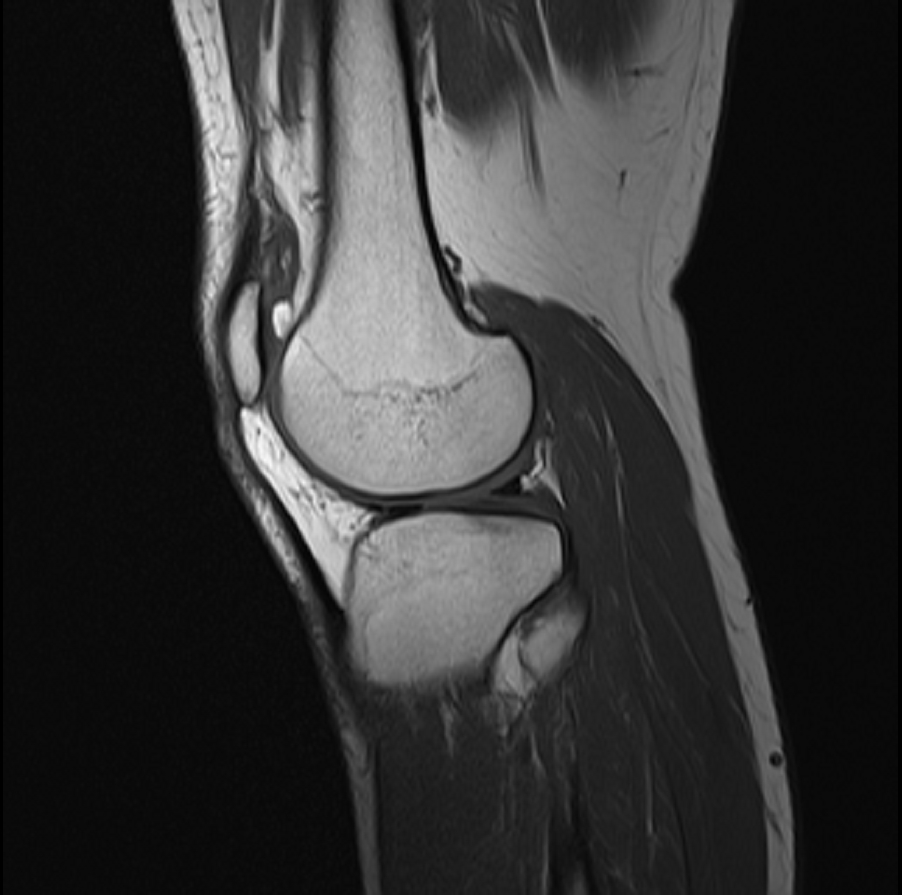
\includegraphics[height=56mm]{img/commons/sag_t1.jpg}};
    \begin{scope}[x={(a.south east)}, y={(a.north west)}]
      \draw[them, line width=1.1pt, -{Stealth}] (0.20,0.86) -- (0.41,0.66);
      \node[font=\scriptsize\bfseries, text=white, fill=them, inner sep=1.5pt, anchor=south] at (0.20,0.86) {bone marrow: bright};
    \end{scope}
  \end{tikzpicture}
  \caption{\textbf{T1}: fat is bright. The bone marrow (fatty) looks white; fluid is dark. Good for anatomy and
  fracture lines.}
\end{subfigure}\hspace{6mm}
\begin{subfigure}[t]{0.42\linewidth}\centering
  \begin{tikzpicture}
    \node[anchor=south west, inner sep=0] (b) at (0,0) {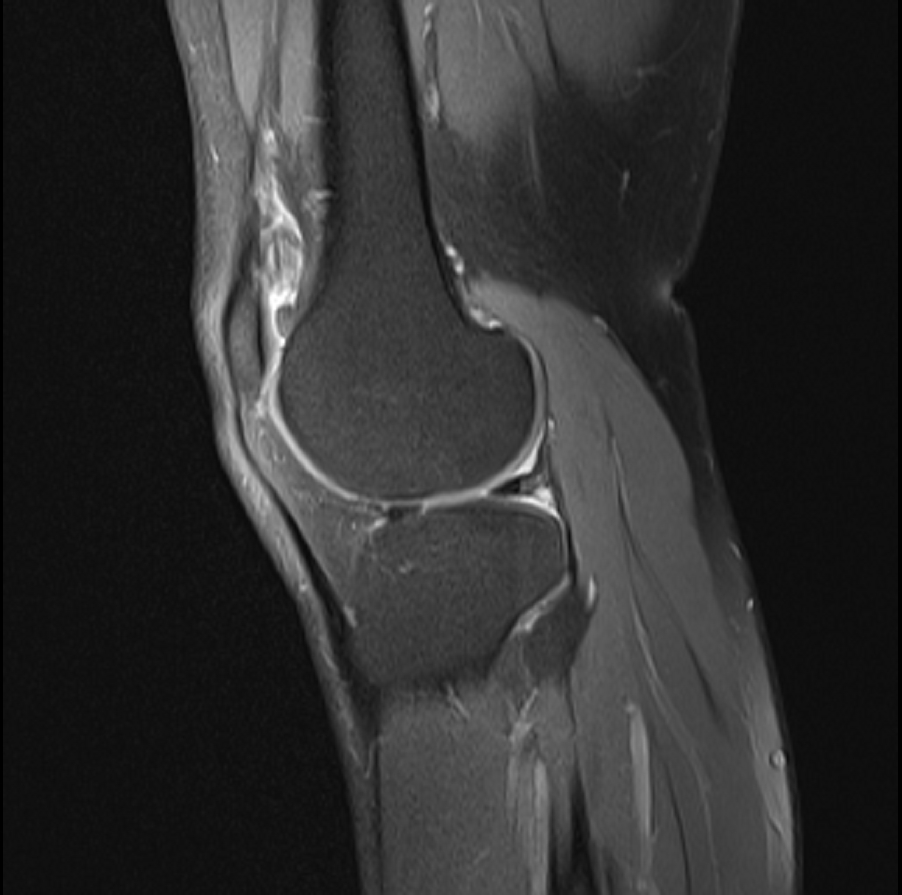
\includegraphics[height=56mm]{img/commons/sag_pd_fs.jpg}};
    \begin{scope}[x={(b.south east)}, y={(b.north west)}]
      \draw[us, line width=1.1pt, -{Stealth}] (0.12,0.86) -- (0.28,0.69);
      \node[font=\scriptsize\bfseries, text=white, fill=us, inner sep=1.5pt, anchor=south] at (0.12,0.86) {fluid: bright};
      \draw[them, line width=1.1pt, -{Stealth}] (0.72,0.86) -- (0.47,0.60);
      \node[font=\scriptsize\bfseries, text=white, fill=them, inner sep=1.5pt, anchor=south] at (0.72,0.86) {marrow: grey};
    \end{scope}
  \end{tikzpicture}
  \caption{\textbf{PD fat-suppressed}: fat is switched off. Marrow turns grey; fluid and swelling stand out white.
  Good for tears, effusion, bone bruises.}
\end{subfigure}
\caption{The same knee, the same slice position, two sequences. Images: Ptrump16, Wikimedia Commons, CC BY-SA 4.0.}
\label{fig:t1pd}
\end{figure}

\begin{center}\small
\begin{tabular}{lcc}
\toprule
Tissue & T1 & fluid-sensitive, fat-suppressed \\
\midrule
fat (under the skin, bone marrow) & \textbf{bright} & dark \\
fluid (effusion, cysts) & dark & \textbf{bright} \\
swelling / edema (bone bruise) & greyish & \textbf{bright} \\
ligaments, tendons, menisci & dark & dark (a tear = a bright line) \\
cartilage, muscle & grey & grey \\
\bottomrule
\end{tabular}
\end{center}

\begin{keyidea}
Most of the 12 findings are ``water where it should not be'': fluid in the joint, swelling in the bone, fluid
seeping into a torn ligament or meniscus. A \textbf{fluid-sensitive, fat-suppressed} series makes exactly that
bright. That is why our pipeline used those series first.
\end{keyidea}

\begin{wordcheck}
\term{PD} (proton density), \term{T1}, \term{T2}: names of sequences. \term{Fat suppression} (``fat-sat'',
``FS''): a trick that removes the fat signal. \term{Fluid-sensitive}: a sequence where water is bright (PD or T2,
usually with fat suppression). The competition's \code{train\_series.csv} tells you, for every series, its plane,
whether it is fluid-sensitive and whether fat is suppressed.
\end{wordcheck}

\section{A typical knee exam}

\begin{center}\small
\begin{tabular}{llll}
\toprule
Series & Plane & Sequence & Used by us? \\
\midrule
\textbf{sag fluid} & sagittal & PD fat-suppressed & \cmark\ role \code{sag\_fs} \\
\textbf{cor fluid} & coronal & PD or T2 fat-suppressed & \cmark\ role \code{cor\_fs} \\
\textbf{ax fluid} & axial & PD fat-suppressed & \cmark\ role \code{ax\_fs} \\
sag structural & sagittal & T1 or PD without fat suppression & \xmark\ (the winners did) \\
cor structural & coronal & T1 & \xmark\ (the winners did) \\
\bottomrule
\end{tabular}
\end{center}
The training set has 24,371 series for 4,407 exams: about \textbf{5.5 series per exam}. Sites differ: some scan
more, some fewer, and they name and store them differently.

\section{Voxels are not cubes}

\begin{figure}[H]
\centering
\begin{tikzpicture}[x={(1cm,0cm)}, y={(0.5cm,0.35cm)}, z={(0cm,1cm)}]
  % a thin, tall voxel
  \foreach \f in {{(0,0,0)--(0.4,0,0)--(0.4,0,3.5)--(0,0,3.5)--cycle},
                  {(0.4,0,0)--(0.4,0.4,0)--(0.4,0.4,3.5)--(0.4,0,3.5)--cycle},
                  {(0,0,3.5)--(0.4,0,3.5)--(0.4,0.4,3.5)--(0,0.4,3.5)--cycle}}
    \filldraw[fill=keyfill, draw=accent, line width=0.6pt] \f;
  \node[font=\scriptsize, anchor=north] at (0.2,0,-0.1) {0.4\,mm};
  \node[font=\scriptsize, anchor=west] at (0.65,0.4,1.75) {3.5\,mm};
  \node[font=\footnotesize, align=center] at (0.4,0,-0.9) {one voxel\\ (3D pixel)};
  % a reformat: sagittal stack viewed from the front is blocky
  \begin{scope}[xshift=4cm]
    \foreach \i in {0,...,7} {
      \pgfmathsetmacro{\g}{50+30*sin(\i*45)}
      \fill[dark!\g] ({\i*0.45},0,0) rectangle ({\i*0.45+0.43},0,3.5);
    }
    \node[font=\footnotesize, align=center] at (1.8,0,-0.9) {the same stack seen from the front:\\ only 8 thick columns};
  \end{scope}
\end{tikzpicture}
\caption{Within a slice the detail is fine; across slices it is about ten times coarser. Turning a sagittal stack
into a front view gives a blocky picture.}
\end{figure}

\begin{why}
This is why most solutions (ours and the winners') use \textbf{2D image models on single slices or on a few
neighbouring slices} (``2.5D'', Chapter~\ref{ch:toolbox}) instead of true 3D models, and why the exam includes
three directions: each direction is sharp where the others are coarse.
\end{why}

\section{MRI has no units}

In a CT scan, water is always 0 on the brightness scale. In MRI the raw numbers depend on the scanner, the coil,
the sequence and the patient. Only \emph{relative} brightness inside one series means anything.

\begin{figure}[H]
\centering
\begin{tikzpicture}
\begin{groupplot}[group style={group size=2 by 1, horizontal sep=18mm}, width=6.6cm, height=4.3cm,
    ytick=\empty, axis x line*=bottom, axis y line=none, xlabel style={font=\footnotesize}]
  \nextgroupplot[xlabel={raw pixel value}, xmin=0, xmax=4000, xtick={0,1000,2000,3000,4000},
                 scaled x ticks=false, xticklabel style={font=\scriptsize}]
    \addplot[us, line width=1.2pt, domain=0:4000, samples=120] {exp(-((x-700)/200)^2) + 0.5*exp(-((x-1300)/250)^2)};
    \addplot[them, line width=1.2pt, domain=0:4000, samples=120] {exp(-((x-1800)/450)^2) + 0.5*exp(-((x-3000)/500)^2)};
    \node[font=\scriptsize, text=us] at (axis cs:700,1.12) {scanner A};
    \node[font=\scriptsize, text=them] at (axis cs:2400,1.12) {scanner B};
  \nextgroupplot[xlabel={after per-series scaling to 0--255}, xmin=0, xmax=255, xtick={0,128,255},
                 xticklabel style={font=\scriptsize}]
    \addplot[us, line width=1.2pt, domain=0:255, samples=120] {exp(-((x-90)/25)^2) + 0.5*exp(-((x-170)/30)^2)};
    \addplot[them, line width=1.2pt, dashed, domain=0:255, samples=120] {exp(-((x-95)/26)^2) + 0.5*exp(-((x-172)/30)^2)};
\end{groupplot}
\end{tikzpicture}
\caption{The same two tissues on two scanners (schematic). Raw values are not comparable (left). Scaling every
series by its own percentiles lines them up (right). Chapter~\ref{ch:cache} shows how we did it.}
\end{figure}

\begin{checkpoint}
\begin{itemize}
\done I can name the three directions and say what each one is good for.
\done I know why fluid-sensitive, fat-suppressed series matter for this task.
\quiz Q3.1: On a T1 image, is a bone bruise easy to see? On a fat-suppressed PD image?
\quiz Q3.2: Why can't you use one fixed brightness rule (``above 1,000 = fluid'') for all exams?
\quiz Q3.3: A model sees only sagittal images. Which finding might it struggle with most, and why?
\end{itemize}
\end{checkpoint}
